\chapter{Resultados}
\label{cap:4-resultados}

\section{Estudio estadístico}

Esta sección presenta los resultados fruto de realizar el estudio estadístico, con el objetivo de averiguar cuales eran los mejores parámetros de los propuestos en el capítulo anterior para que el algoritmo evolutivo consiguiera mejores resultados. Se evalúa cada instancia de las mencionadas en la sección~\ref{subsec:instancias} por separado, aportando un conjunto de gráficas de la evolución del fitness para cada conjunto de parámetros evaluado y una tabla con los resultados numéricos de la comparación entre sí de todos los conjuntos, para averiguar si existe una diferencia estadística en los resultados ofrecidos.

\subsection{Instancia S\textsubscript{4}: <<anchieta\_tls\_interior\_lane\_always\_green>>}


Con respecto a los resultados del estudio estadístico de la primera instancia, se puede comprobar en la Figura~\ref{fig:estudio:anchieta_tls_interior_lane_always_green} la evolución del fitness para cada una de las cuatro configuraciones que se plantearon para la instancia. 

Las gráficas revelan claramente un incremento del fitness cuando la población es de 50 individuos, independientemente del cruce empleado, pese a que la mejoría no es especialmente abundante. Así pues, para determinar cual configuración es la mejor, hay que referirse a la Tabla~\ref{tab:estudio:anchieta_tls_interior_lane_always_green}. Aquí figuran todas las configuraciones enfrentadas entre sí en parejas.

En dicha tabla se puede apreciar como, al enfrentar a las configuraciones entre sí, la combinación de cruce \texttt{UniformCrossover} y población 50 se coloca como la mejor de todas, puesto que <<ganó>> tres de los <<enfrentamientos>> contra el resto de las configuraciones, revelándose así como el conjunto de parámetros del algoritmo evolutivo que ofrecen mejores resultados. En segunda posición queda el conjunto \texttt{OnePointCrossover} y población 50, al haber ganado solo dos de los enfrentamientos. Finalmente, puede apreciarse como no existe ninguna diferencia en emplear una configuración que tenga 10 individuos con cualquier tipo de cruce.


\begin{figure}[h]
    \centering
    \begin{subfigure}[t]{.49\textwidth}
      \centering
      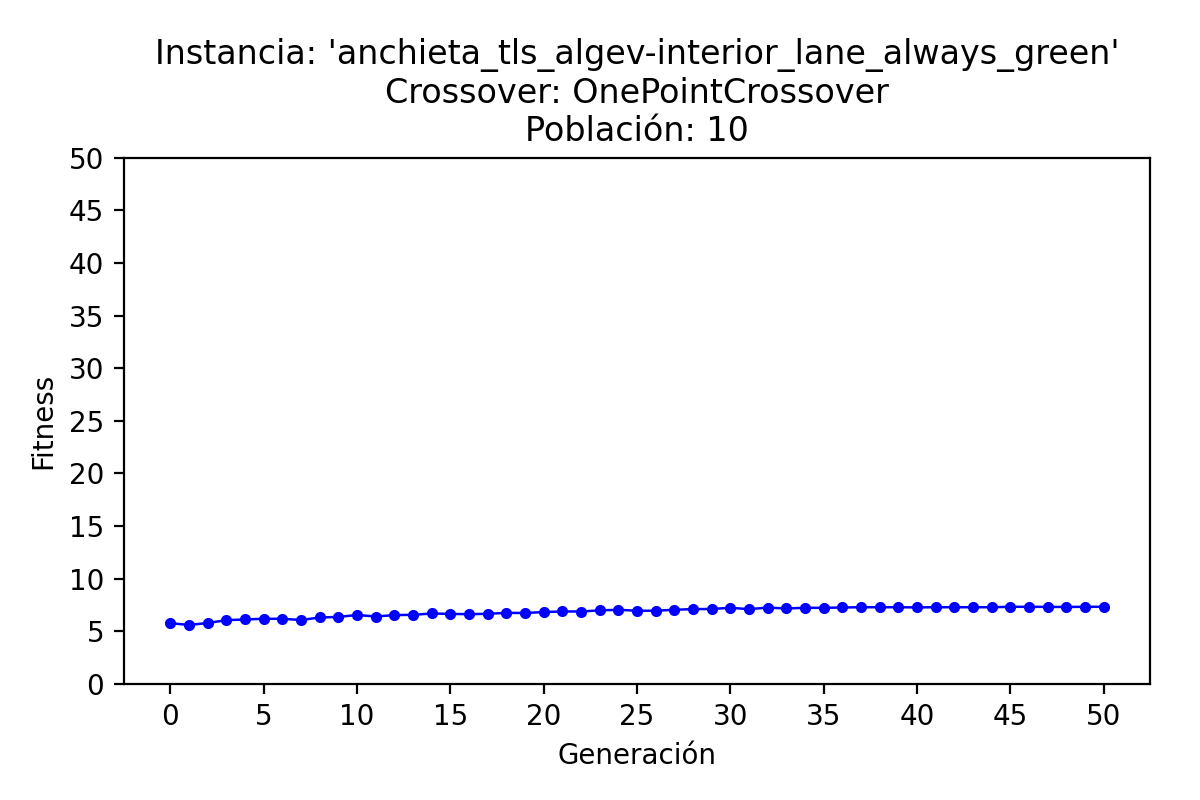
\includegraphics[width=\textwidth]{report/images/estudio/anchieta_tls_algev-interior_lane_always_green-OnePointCrossover-10.png}
    \end{subfigure}
    \hfill
    \begin{subfigure}[t]{.49\textwidth}
      \centering
      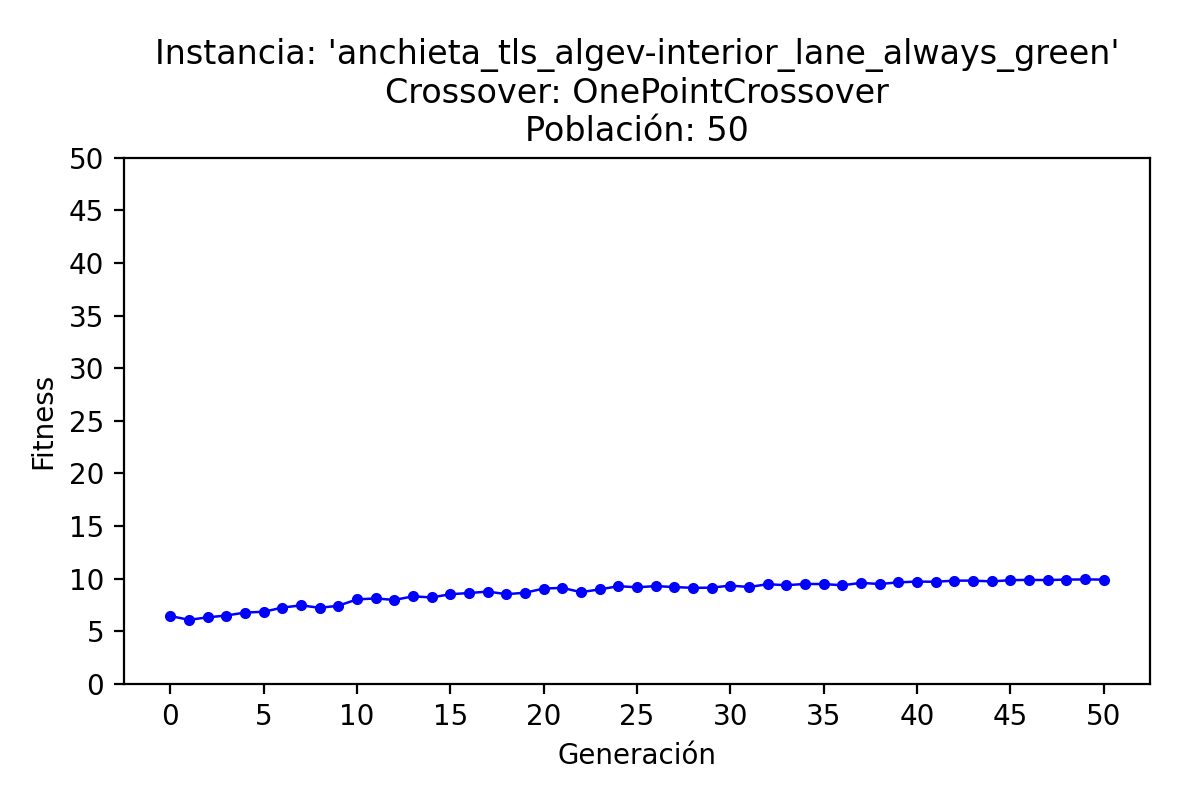
\includegraphics[width=\textwidth]{report/images/estudio/anchieta_tls_algev-interior_lane_always_green-OnePointCrossover-50.png}
    \end{subfigure}
    \vspace{0.7cm}
    \begin{subfigure}[t]{.49\textwidth}
      \centering
      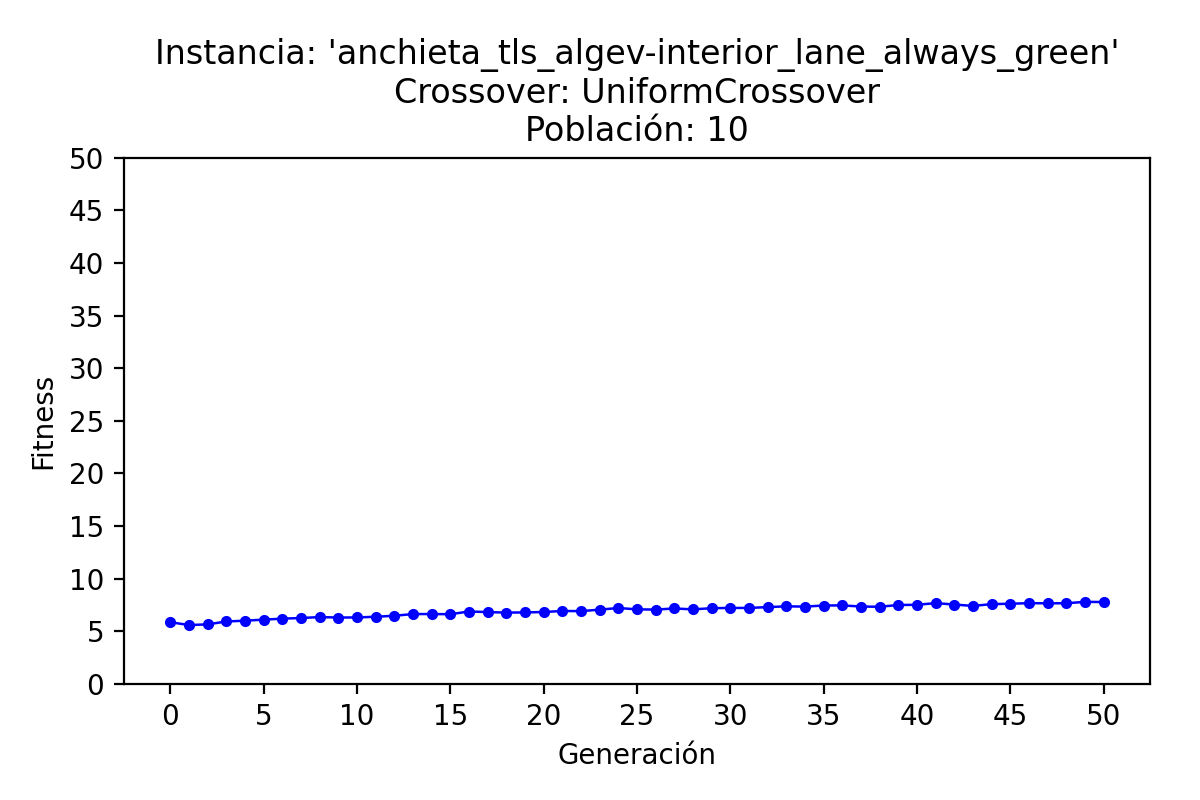
\includegraphics[width=\textwidth]{report/images/estudio/anchieta_tls_algev-interior_lane_always_green-UniformCrossover-10.png}
    \end{subfigure}
    \hfill
    \begin{subfigure}[t]{.49\textwidth}
      \centering
      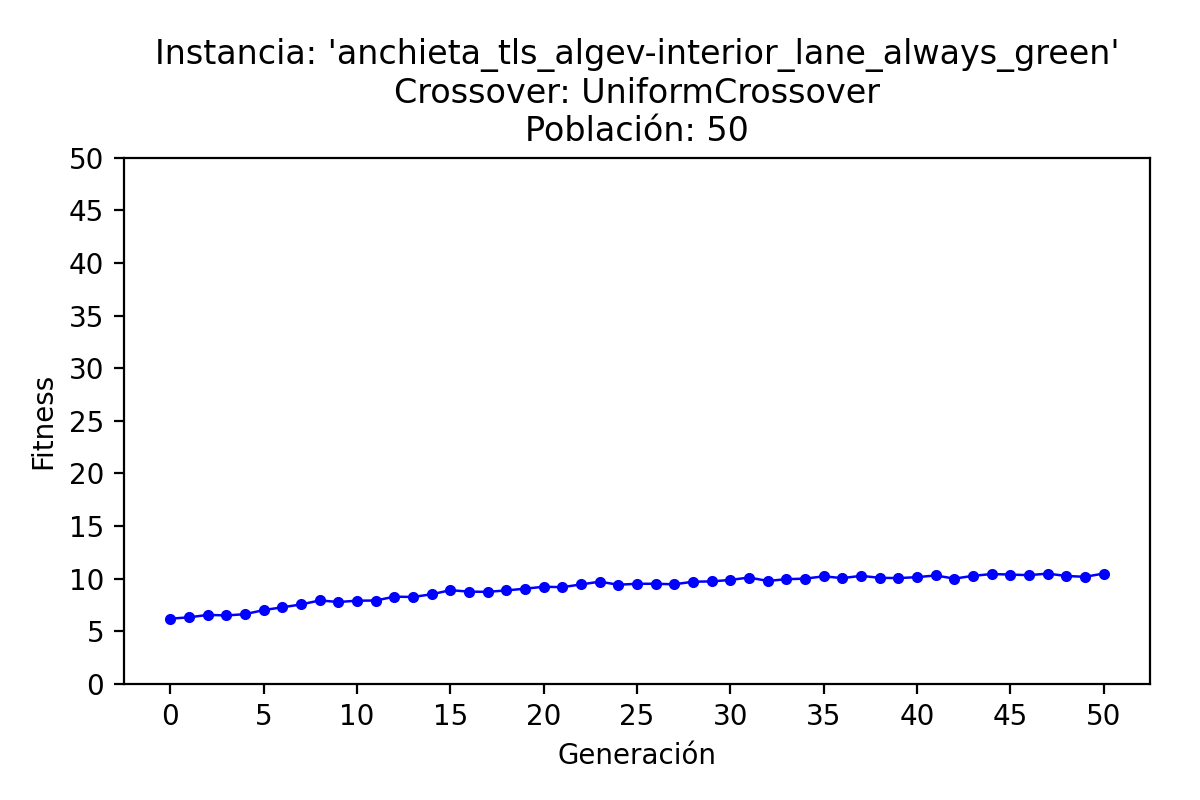
\includegraphics[width=\textwidth]{report/images/estudio/anchieta_tls_algev-interior_lane_always_green-UniformCrossover-50.png}
    \end{subfigure}
    \caption{Evolución del fitness medio entre ejecuciones del mejor candidato de cada generación para la instancia S\textsubscript{4}}
    \label{fig:estudio:anchieta_tls_interior_lane_always_green}
\end{figure}

\subsection{Instancia S\textsubscript{5}: <<anchieta\_tls\_interior\_lane\_changes>>}

Lo cierto es que el estudio de esta instancia arroja resultados similares a los de la instancia anterior. El estudio de la evolución del fitess, que puede apreciarse en la Figura~\ref{fig:estudio:anchieta_tls_interior_lane_changes}, parece resaltar que, al igual que con la instancia anterior, el fitness mejora al usar una población mayor. Sin embargo, esta instancia proporciona, de manera general, un valor de fitness más alto que la anterior; y en el caso de las comparativas entre cruces, la diferencia en el valor del fitness es más acusada.

Observando los resultados de la evaluación por parejas de las diferentes configuraciones de la Tabla~\ref{tab:estudio:anchieta_tls_interior_lane_changes}, los resultados quedan idénticos a los de la instancia anterior, terminando como ganador el conjunto de parámetros que emplea el cruce \texttt{UniformCrossover} y una población de 50 individuos. En segundo lugar, queda el conjunto \texttt{OnePointCrossover} y población 50 individuos; y de la misma manera, se comprueba que no hay diferencia en emplear uno u otro cruce cuando la población es de 10 invididuos.

\begin{figure}[h]
    \centering
    \begin{subfigure}[t]{.49\textwidth}
      \centering
      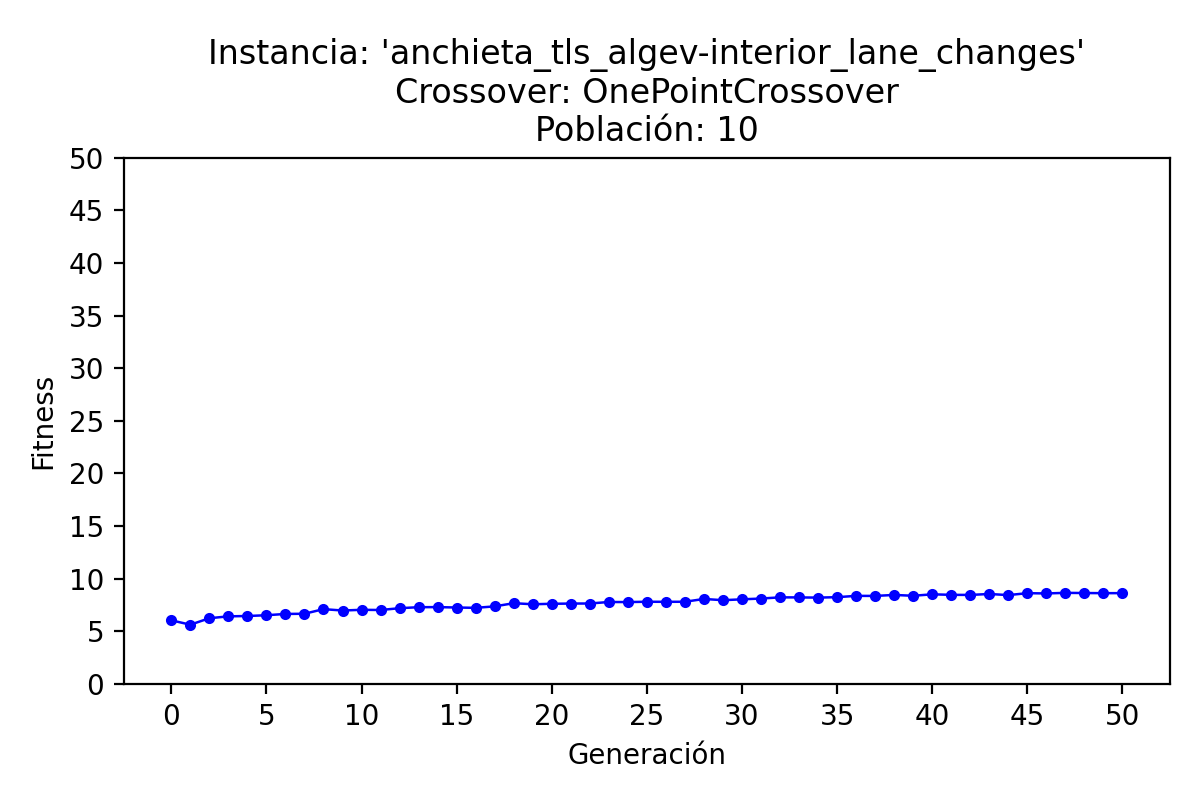
\includegraphics[width=\textwidth]{report/images/estudio/anchieta_tls_algev-interior_lane_changes-OnePointCrossover-10.png}
    \end{subfigure}
    \hfill
    \begin{subfigure}[t]{.49\textwidth}
      \centering
      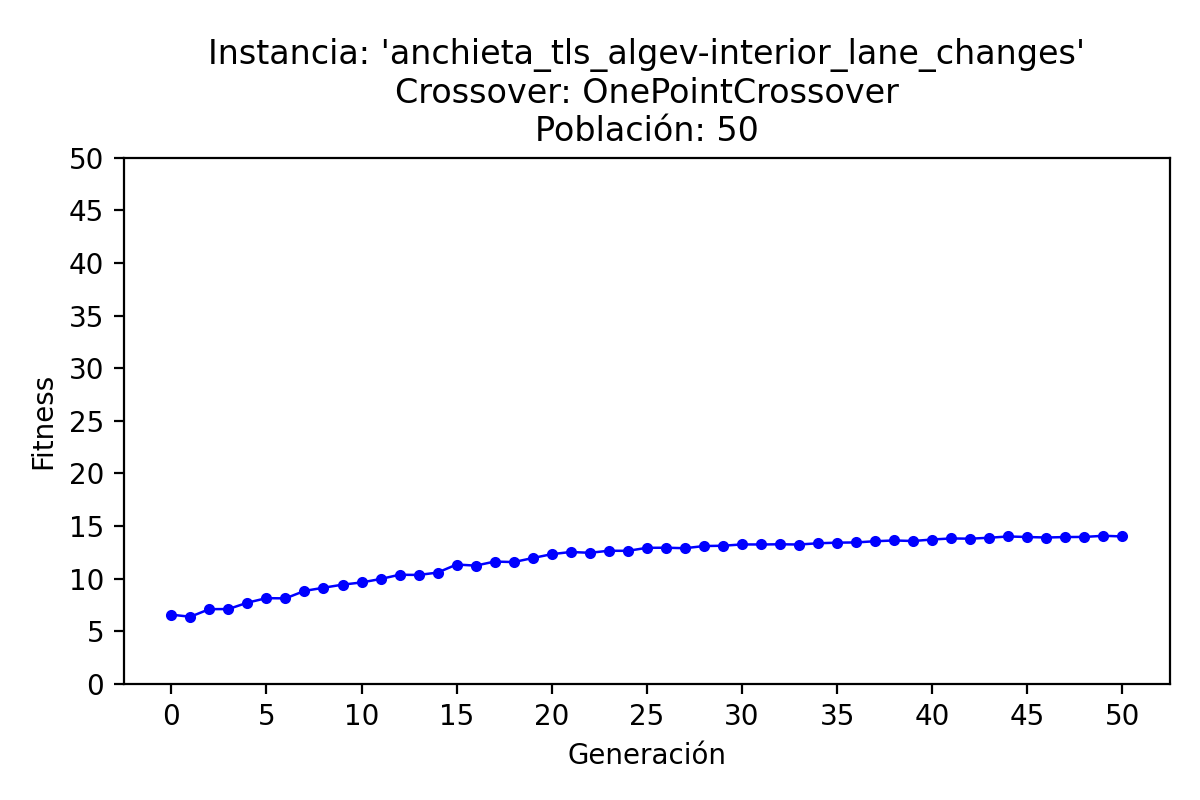
\includegraphics[width=\textwidth]{report/images/estudio/anchieta_tls_algev-interior_lane_changes-OnePointCrossover-50.png}
    \end{subfigure}
    \vspace{0.7cm}
    \begin{subfigure}[t]{.49\textwidth}
      \centering
      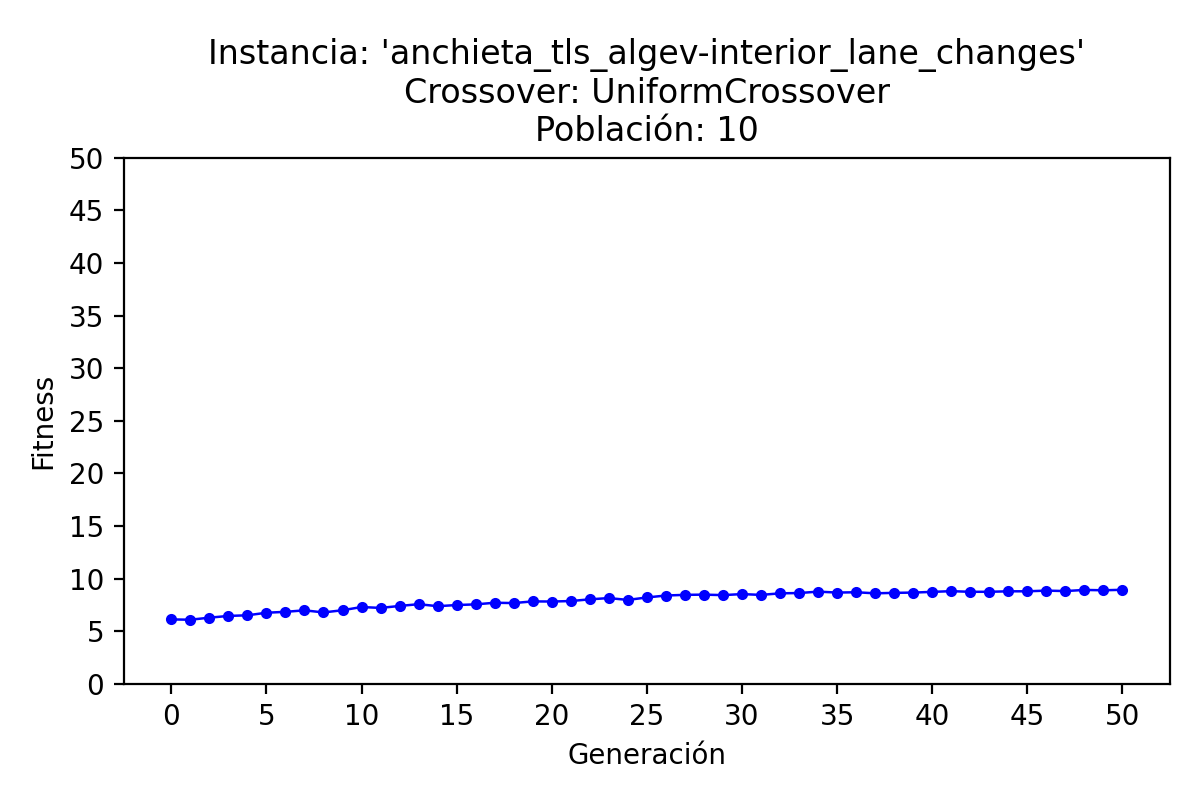
\includegraphics[width=\textwidth]{report/images/estudio/anchieta_tls_algev-interior_lane_changes-UniformCrossover-10.png}
    \end{subfigure}
    \hfill
    \begin{subfigure}[t]{.49\textwidth}
      \centering
      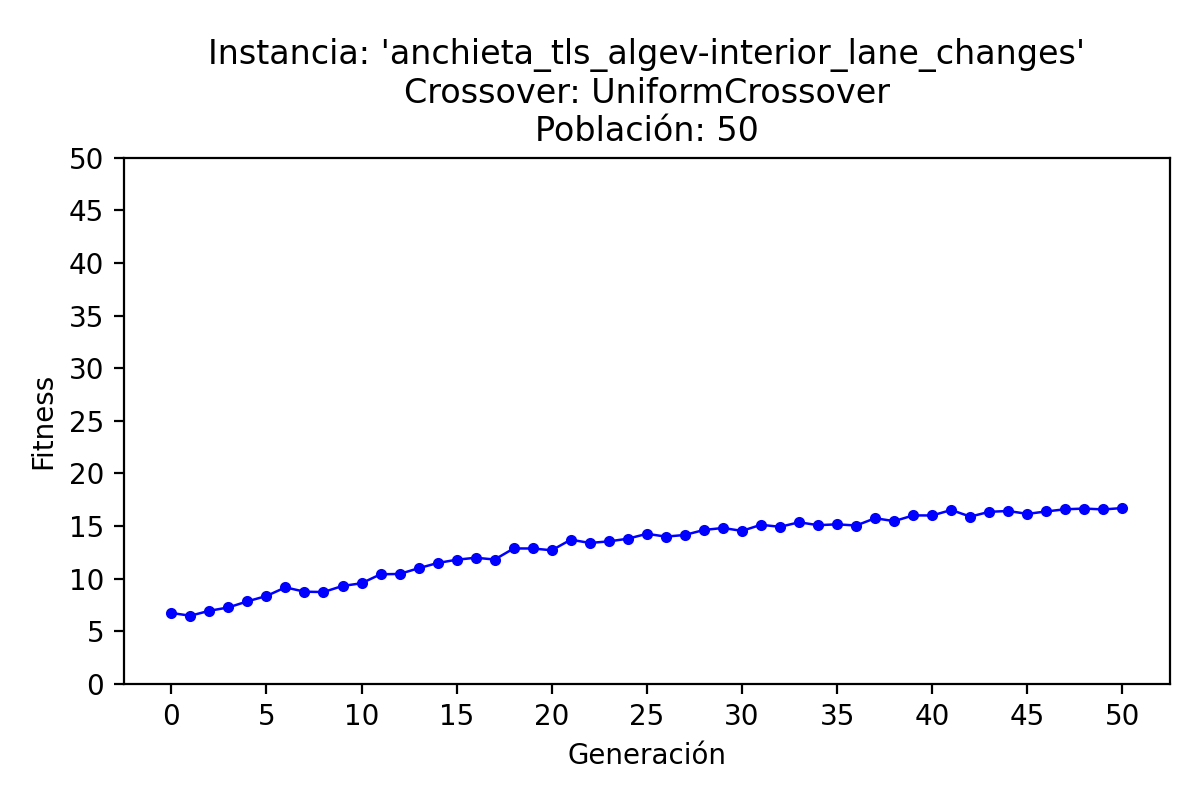
\includegraphics[width=\textwidth]{report/images/estudio/anchieta_tls_algev-interior_lane_changes-UniformCrossover-50.png}
    \end{subfigure}
    \caption{Evolución del fitness medio entre ejecuciones del mejor candidato de cada generación para la instancia S\textsubscript{5}}
    \label{fig:estudio:anchieta_tls_interior_lane_changes}
\end{figure}



\subsection{Instancia S\textsubscript{6}: <<anchieta\_tls\_few\_pedestrians>>}

En comparación con las anteriores, los resultados de la evaluación del fitness de esta instancia (Figura~\ref{fig:estudio:anchieta_tls_special_few_pedestrians}) arrojan resultados mucho mayores; por lo cual se aprecia que la utilización de menos semáforos redunda en un incremento bastante acusado del fitness. Asímismo, y en consonancia con las evaluaciones anteriores, la diferencia en la población se cristaliza una vez más como causante de un incremento en el fitness en el caso de ambos cruces, dando mejores resultados la utilización 50 individuos por generación.

Sin embargo, observando los resultados de la evaluación de los conjuntos de parámetros (Tabla~\ref{tab:estudio:anchieta_tls_special_few_pedestrians}), se puede apreciar como los conjuntos \texttt{OnePointCrossover/Pob50} y \texttt{UniformCrossover/Pob50} llegan a un empate en el cual ambos han ganado (y perdido) la misma cantidad de veces en las evaluaciones con otros conjuntos, además de que no se aprecia diferencia estadística entre uno y otro. Así pues, la conclusión es que realmente no hay diferencia entre emplear cualquiera de los dos, puesto que brindaran resultados extremadamente parecidos.

\begin{figure}[h]
    \centering
    \begin{subfigure}[t]{.49\textwidth}
      \centering
      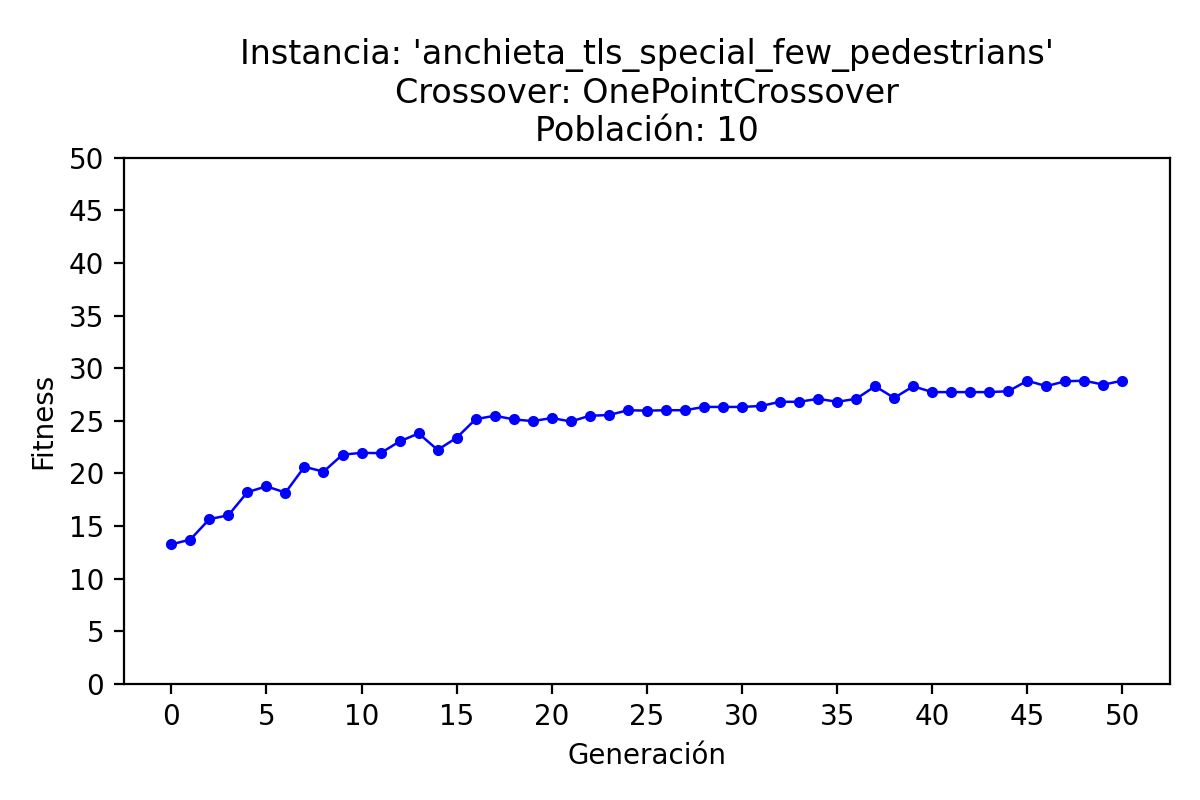
\includegraphics[width=\textwidth]{report/images/estudio/anchieta_tls_special_few_pedestrians-OnePointCrossover-10.png}
    \end{subfigure}
    \hfill
    \begin{subfigure}[t]{.49\textwidth}
      \centering
      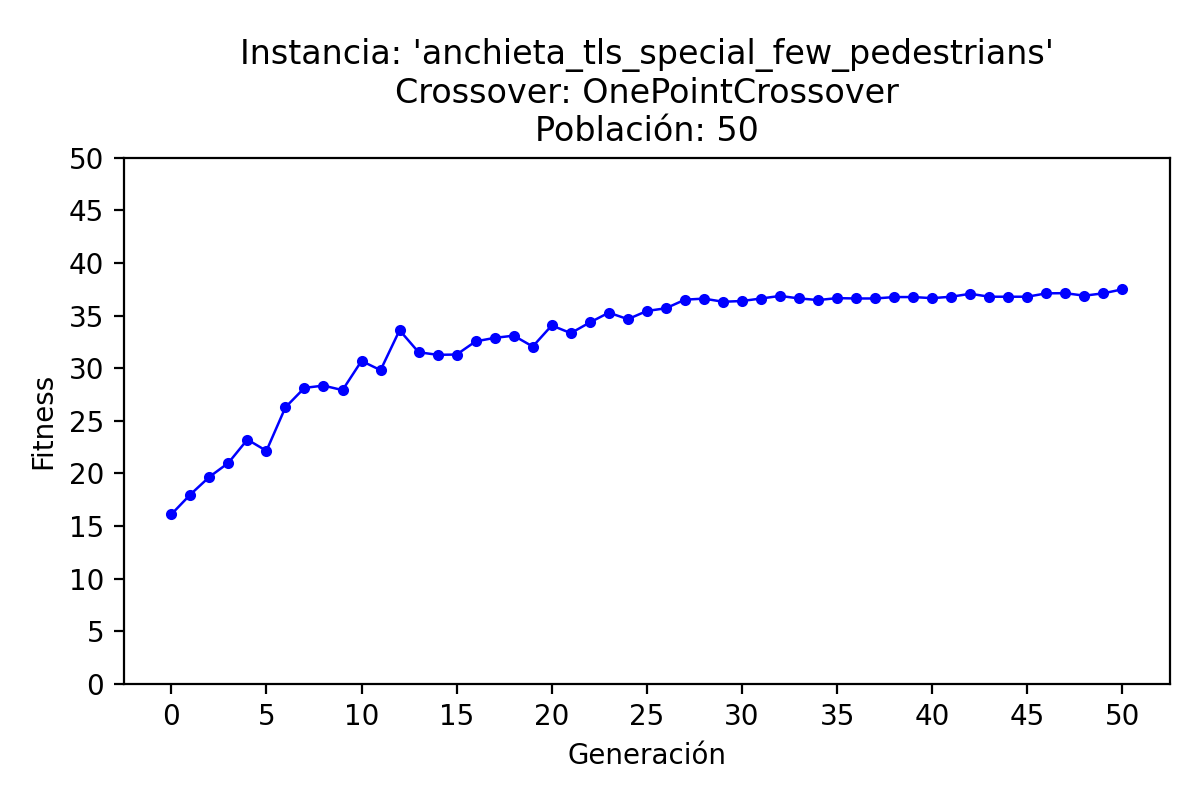
\includegraphics[width=\textwidth]{report/images/estudio/anchieta_tls_special_few_pedestrians-OnePointCrossover-50.png}
    \end{subfigure}
    \vspace{0.7cm}
    \begin{subfigure}[t]{.49\textwidth}
      \centering
      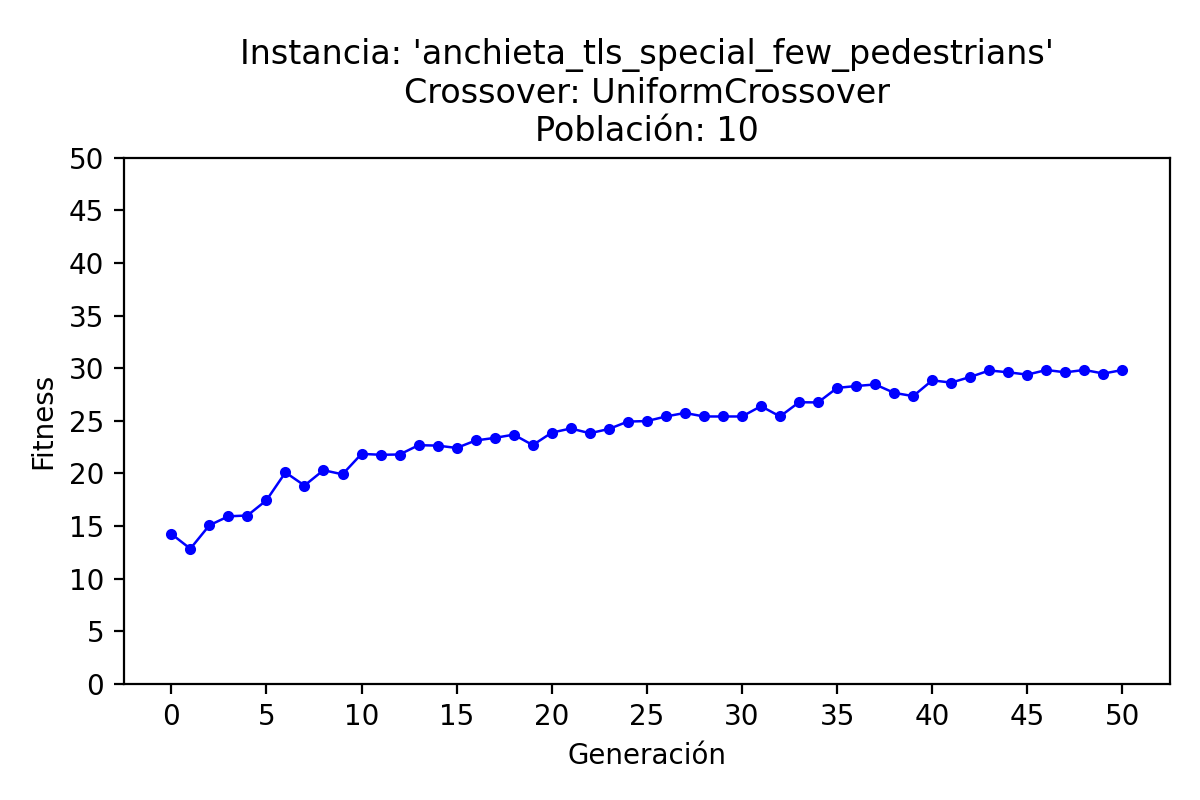
\includegraphics[width=\textwidth]{report/images/estudio/anchieta_tls_special_few_pedestrians-UniformCrossover-10.png}
    \end{subfigure}
    \hfill
    \begin{subfigure}[t]{.49\textwidth}
      \centering
      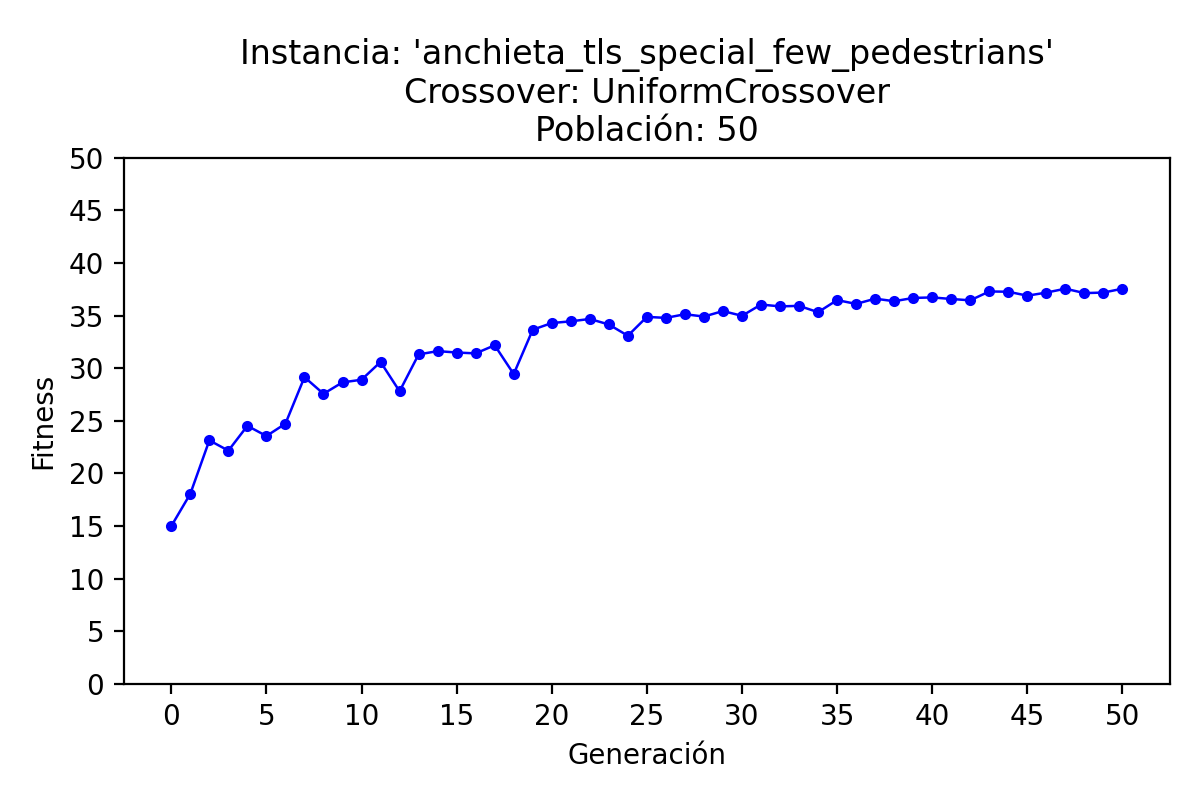
\includegraphics[width=\textwidth]{report/images/estudio/anchieta_tls_special_few_pedestrians-UniformCrossover-50.png}
    \end{subfigure}
    \caption{Evolución del fitness medio entre ejecuciones del mejor candidato de cada generación para la instancia S\textsubscript{6}}
    \label{fig:estudio:anchieta_tls_special_few_pedestrians}
\end{figure}



\subsection{Instancia S\textsubscript{7}: <<anchieta\_tls\_many\_pedestrians>>}

La evaluación del fitness de cada conjunto de parámetros empleado en esta instancia ofrece resultados interesantes si se compara con la anterior, puesto que es fácil apreciar una reducción considerable del fitness en todos los casos, tal y como se puede apreciar en la Figura~\ref{fig:estudio:anchieta_tls_special_many_pedestrians}.  

Observando los resultados de la competición entre sí de cada conjunto (Tabla~\ref{tab:estudio:anchieta_tls_special_many_pedestrians}), se comprueba que los resultados son idénticos a los de la instancia anterior, con un empate entre los conjuntos \texttt{OnePointCrossover/Pob50} y \texttt{UniformCrossover/Pob50}; de modo que no hay diferencia entre emplear uno u otro.

\begin{figure}[h]
    \centering
    \begin{subfigure}[t]{.49\textwidth}
      \centering
      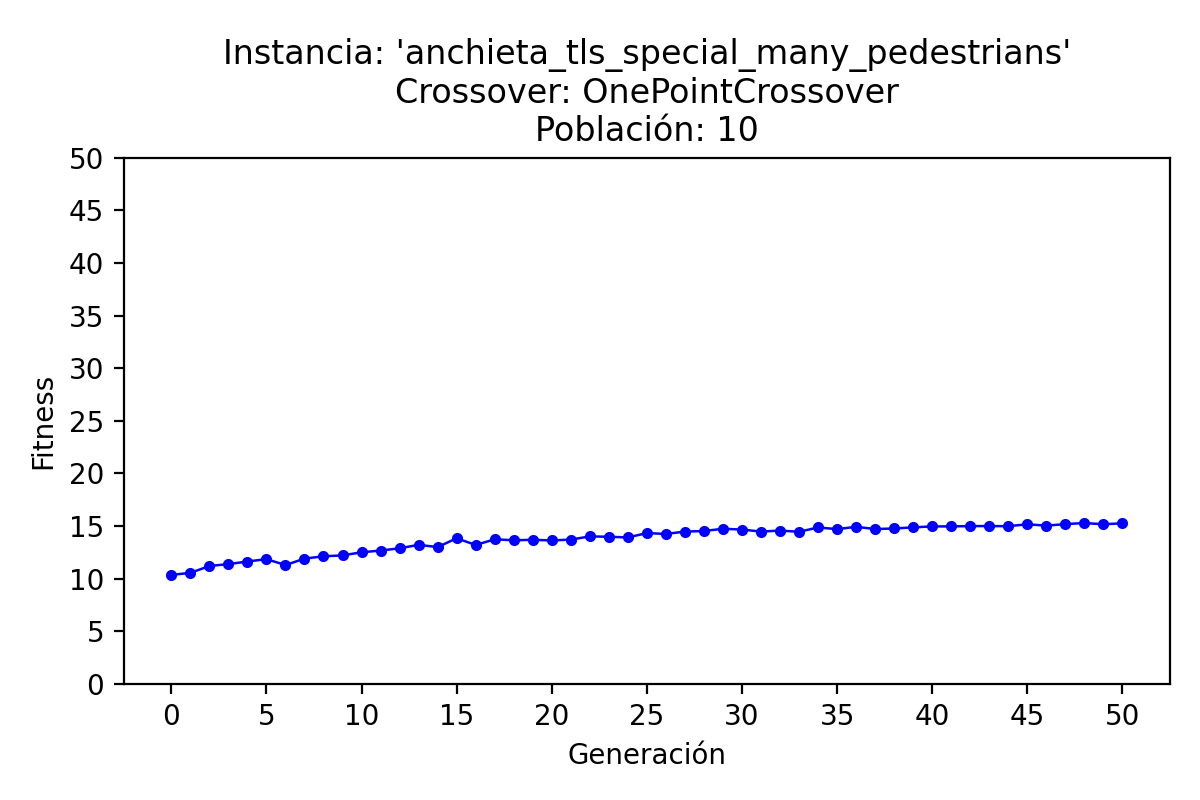
\includegraphics[width=\textwidth]{report/images/estudio/anchieta_tls_special_many_pedestrians-OnePointCrossover-10.png}
    \end{subfigure}
    \hfill
    \begin{subfigure}[t]{.49\textwidth}
      \centering
      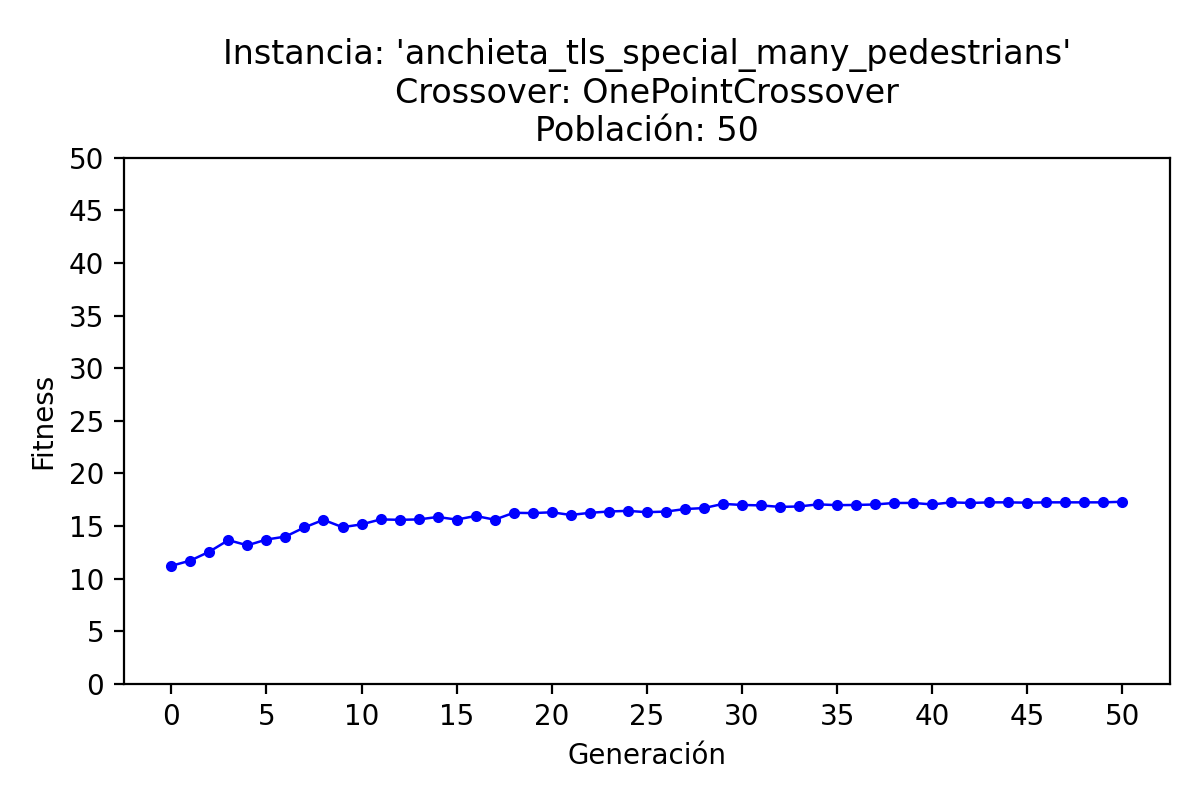
\includegraphics[width=\textwidth]{report/images/estudio/anchieta_tls_special_many_pedestrians-OnePointCrossover-50.png}
    \end{subfigure}
    \vspace{0.7cm}
    \begin{subfigure}[t]{.49\textwidth}
      \centering
      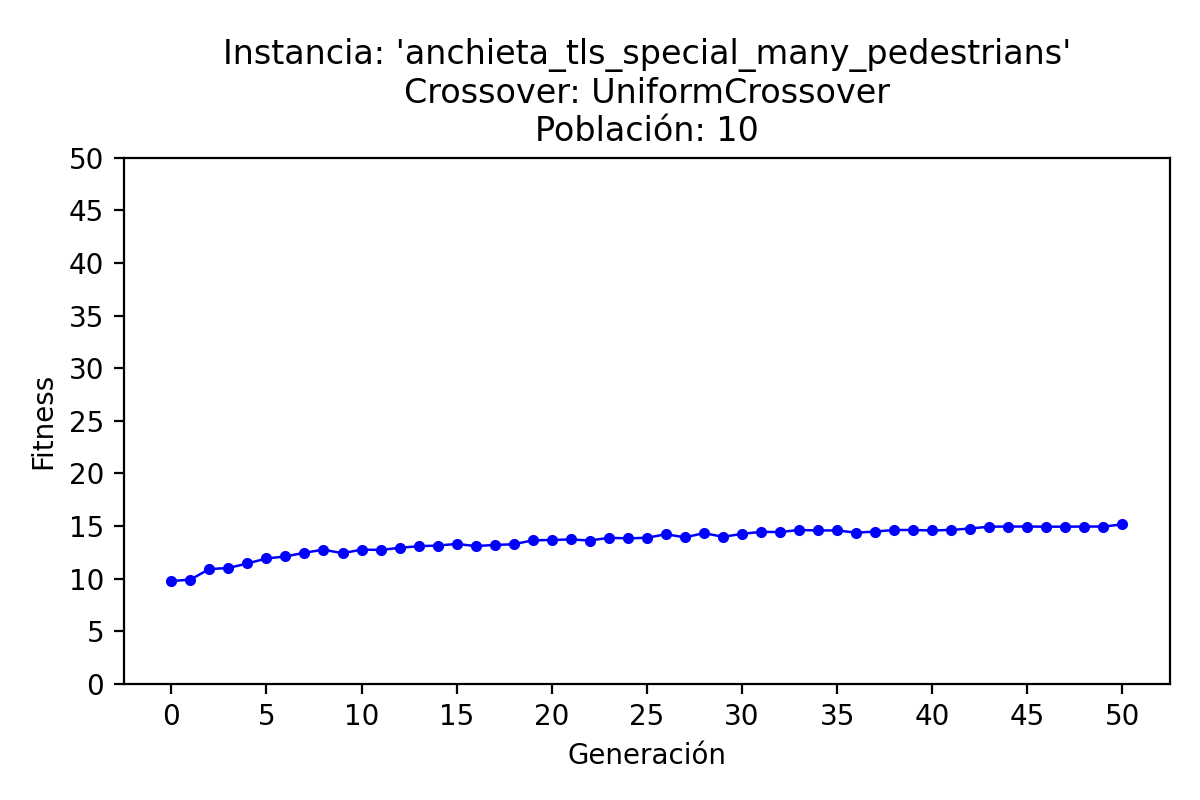
\includegraphics[width=\textwidth]{report/images/estudio/anchieta_tls_special_many_pedestrians-UniformCrossover-10.png}
    \end{subfigure}
    \hfill
    \begin{subfigure}[t]{.49\textwidth}
      \centering
      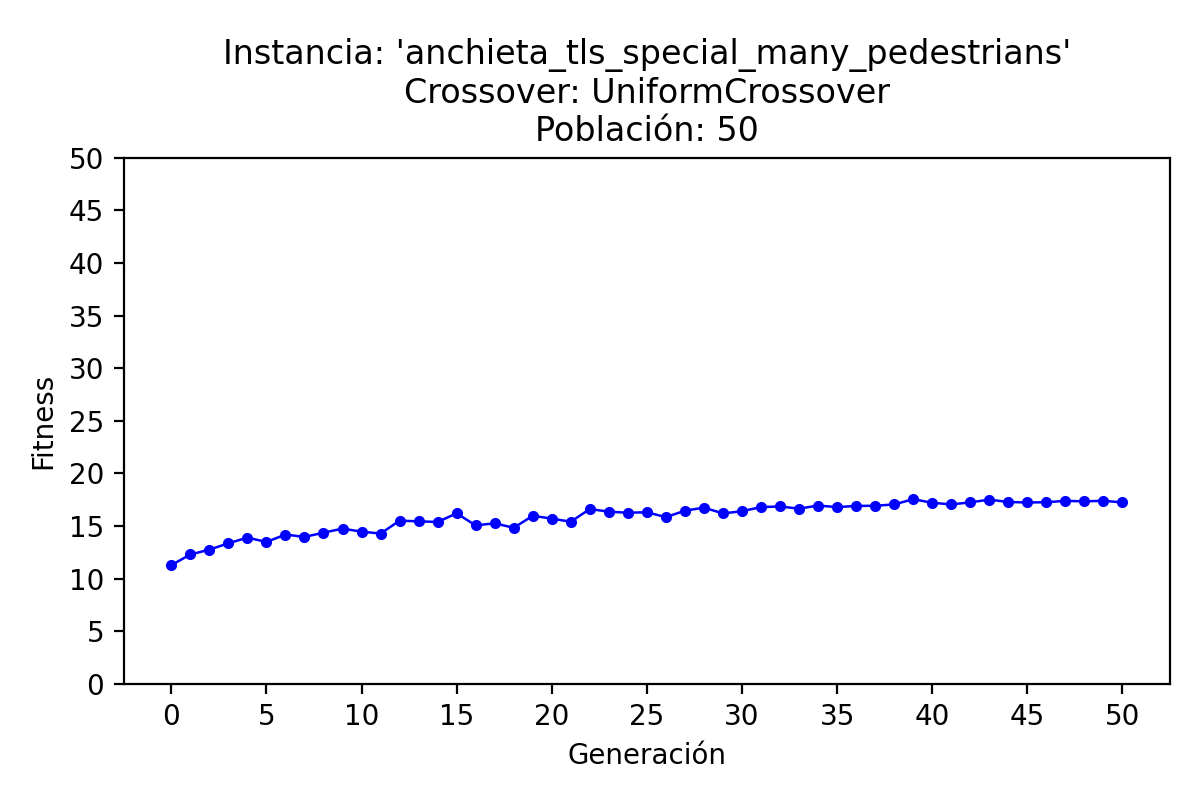
\includegraphics[width=\textwidth]{report/images/estudio/anchieta_tls_special_many_pedestrians-UniformCrossover-50.png}
    \end{subfigure}
    \caption{Evolución del fitness medio entre ejecuciones del mejor candidato de cada generación para la instancia S\textsubscript{7}}
    \label{fig:estudio:anchieta_tls_special_many_pedestrians}
\end{figure}


\subsection{Análisis de los resultados}

Realizada una evaluación de las configuraciones anteriores, para la simulación se emplearán las instancias obtenidas del algoritmo evolutivo con los siguientes conjuntos de parámetros:

\begin{itemize}
    \item \textbf{anchieta\_tls\_interior\_lane\_always\_green:}: \texttt{UniformCrossover/Pob50}
    \item \textbf{anchieta\_tls\_interior\_lane\_changes:} \texttt{UniformCrossover/Pob50}
    \item \textbf{anchieta\_tls\_few\_pedestrians:} \texttt{UniformCrossover/Pob50}
    \item \textbf{anchieta\_tls\_many\_pedestrians:} \texttt{UniformCrossover/Pob50}
\end{itemize}



% TABLAS

\begin{sidewaystable}[h]
    \bigskip\bigskip
    \caption{}
    \label{tab:estudio:anchieta_tls_special_few_pedestrians}
    \resizebox{\textwidth}{!}{\begin{tabular}{lllllll}
    \hline
    \multicolumn{7}{c}{\textbf{anchieta\_tls\_few\_pedestrians}}                                                                                                                                                                                             \\ \hline
    \multicolumn{1}{c}{\multirow{2}{*}{\textit{Conjuntos de parámetros 1 y 2}}}        & \multicolumn{2}{c}{\textit{Media}}            & \multicolumn{2}{c}{\textit{Mediana}}          & \multicolumn{1}{c}{\multirow{2}{*}{\textit{p-value}}} & \multicolumn{1}{c}{\multirow{2}{*}{\textit{Ganador}}} \\ \cline{2-5}
    \multicolumn{1}{c}{}                                                & \multicolumn{1}{c}{1} & \multicolumn{1}{c}{2} & \multicolumn{1}{c}{1} & \multicolumn{1}{c}{2} & \multicolumn{1}{c}{}                                  & \multicolumn{1}{c}{}                                  \\ \hline
    OnePointCrossover/Pop10 y OnePointCrossover/Pop50                   & 29.45247              & 37.67554              & 27.4298               & 38.05608              & 0.0002177574                                          & OnePointCrossover/Pop50                               \\ \hline
    OnePointCrossover/Pop10 y UniformCrossover/Pop10                    & 29.45247              & 29.88526              & 27.4298               & 28.53967              & 0.8623907                                             & No hay diferencia estadística                         \\ \hline
    OnePointCrossover/Pop10 y UniformCrossover/Pop50                    & 29.45247              & 38.31307              & 27.4298               & 38.35384              & 0.0003900244                                          & UniformCrossover/Pop50                                \\ \hline
    OnePointCrossover/Pop50 y UniformCrossover/Pop10                    & 37.67554              & 29.88526              & 38.05608              & 28.53967              & 0.00180757                                            & OnePointCrossover/Pop50                               \\ \hline
    OnePointCrossover/Pop50 y UniformCrossover/Pop50                    & 37.67554              & 38.31307              & 38.05608              & 38.35384              & 0.4469909                                             & No hay diferencia estadística                         \\ \hline
    UniformCrossover/Pop10 y UniformCrossover/Pop50                     & 29.88526              & 38.31307              & 28.53967              & 38.35384              & 0.001050841                                           & UniformCrossover/Pop50                                \\ \hline
    \end{tabular}}
    
    \bigskip\bigskip
    \caption{}
    \label{tab:estudio:anchieta_tls_special_many_pedestrians}
    \resizebox{\textwidth}{!}{\begin{tabular}{lllllll}
    \hline
    \multicolumn{7}{c}{\textbf{anchieta\_tls\_many\_pedestrians}}                                                                                                                                                                                            \\ \hline
    \multicolumn{1}{c}{\multirow{2}{*}{\textit{Conjuntos de parámetros 1 y 2}}}        & \multicolumn{2}{c}{\textit{Media}}            & \multicolumn{2}{c}{\textit{Mediana}}          & \multicolumn{1}{c}{\multirow{2}{*}{\textit{p-value}}} & \multicolumn{1}{c}{\multirow{2}{*}{\textit{Ganador}}} \\ \cline{2-5}
    \multicolumn{1}{c}{}                                                & \multicolumn{1}{c}{1} & \multicolumn{1}{c}{2} & \multicolumn{1}{c}{1} & \multicolumn{1}{c}{2} & \multicolumn{1}{c}{}                                  & \multicolumn{1}{c}{}                                  \\ \hline
    OnePointCrossover/Pop10 y OnePointCrossover/Pop50                   & 15.3666               & 17.38808              & 15.65755              & 17.53609              & 7.402106e-05                                          & OnePointCrossover/Pop50                               \\ \hline
    OnePointCrossover/Pop10 y UniformCrossover/Pop10                    & 15.3666               & 15.26587              & 15.65755              & 15.11698              & 0.86804                                               & No hay diferencia estadística                         \\ \hline
    OnePointCrossover/Pop10 y UniformCrossover/Pop50                    & 15.3666               & 17.72223              & 15.65755              & 17.9043               & 4.202438e-05                                          & UniformCrossover/Pop50                                \\ \hline
    OnePointCrossover/Pop50 y UniformCrossover/Pop10                    & 17.38808              & 15.26587              & 17.53609              & 15.11698              & 0.001255819                                           & OnePointCrossover/Pop50                               \\ \hline
    OnePointCrossover/Pop50 y UniformCrossover/Pop50                    & 17.38808              & 17.72223              & 17.53609              & 17.9043               & 0.390172                                              & No hay diferencia estadística                         \\ \hline
    UniformCrossover/Pop10 y UniformCrossover/Pop50                     & 15.26587              & 17.72223              & 15.11698              & 17.9043               & 0.0005555893                                          & UniformCrossover/Pop50                                \\ \hline
    \end{tabular}}
\end{sidewaystable}


\begin{sidewaystable}
    \caption{Resultado de la comparación por parejas de la instancia anchieta\_tls\_interior\_lane\_always\_green}
    \label{tab:estudio:anchieta_tls_interior_lane_always_green}
    \resizebox{\textwidth}{!}{\begin{tabular}{lllllll}
    \hline
    \multicolumn{7}{c}{\textbf{anchieta\_tls\_interior\_lane\_always\_green}}                                                                                                                                                                                   \\ \hline
    \multicolumn{1}{c}{\multirow{2}{*}{\textit{Conjuntos de parámetros 1 y 2}}}        & \multicolumn{2}{c}{\textit{Media}}            & \multicolumn{2}{c}{\textit{Mediana}}          & \multicolumn{1}{c}{\multirow{2}{*}{\textit{p-value}}} & \multicolumn{1}{c}{\multirow{2}{*}{\textit{Ganador}}} \\ \cline{2-5}
    \multicolumn{1}{c}{}                                                & \multicolumn{1}{c}{1} & \multicolumn{1}{c}{2} & \multicolumn{1}{c}{1} & \multicolumn{1}{c}{2} & \multicolumn{1}{c}{}                                  & \multicolumn{1}{c}{}                                  \\ \hline
    OnePointCrossover/Pop10 y OnePointCrossover/Pop50                   & 7.364113              & 9.962546              & 7.298901              & 10.05993              & 5.78933e-05                                           & OnePointCrossover/Pop50                               \\ \hline
    OnePointCrossover/Pop10 y UniformCrossover/Pop10                    & 7.364113              & 7.859806              & 7.298901              & 7.632471              & 0.1928009                                             & No hay diferencia estadística                         \\ \hline
    OnePointCrossover/Pop10 y UniformCrossover/Pop50                    & 7.364113              & 11.16813              & 7.298901              & 11.15414              & 0.0001570523                                          & UniformCrossover/Pop50                                \\ \hline
    OnePointCrossover/Pop50 y UniformCrossover/Pop10                    & 9.962546              & 7.859806              & 10.05993              & 7.632471              & 0.0001639967                                          & OnePointCrossover/Pop50                               \\ \hline
    OnePointCrossover/Pop50 y UniformCrossover/Pop50                    & 9.962546              & 11.16813              & 10.05993              & 11.15414              & 0.0101652                                             & UniformCrossover/Pop50                                \\ \hline
    UniformCrossover/Pop10 y UniformCrossover/Pop50                     & 7.859806              & 11.16813              & 7.632471              & 11.15414              & 0.0001570523                                          & UniformCrossover/Pop50                                \\ \hline
    \end{tabular}}
    
    
    
    \bigskip\bigskip
    \caption{Resultado de la comparación por parejas de la instancia anchieta\_tls\_interior\_lane\_changes}
    \label{tab:estudio:anchieta_tls_interior_lane_changes}
    \resizebox{\textwidth}{!}{\begin{tabular}{lllllll}
    \hline
    \multicolumn{7}{c}{\textbf{anchieta\_tls\_interior\_lane\_changes}}                                                                                                                                                                                         \\ \hline
    \multicolumn{1}{c}{\multirow{2}{*}{\textit{Conjuntos de parámetros 1 y 2}}}        & \multicolumn{2}{c}{\textit{Media}}            & \multicolumn{2}{c}{\textit{Mediana}}          & \multicolumn{1}{c}{\multirow{2}{*}{\textit{p-value}}} & \multicolumn{1}{c}{\multirow{2}{*}{\textit{Ganador}}} \\ \cline{2-5}
    \multicolumn{1}{c}{}                                                & \multicolumn{1}{c}{1} & \multicolumn{1}{c}{2} & \multicolumn{1}{c}{1} & \multicolumn{1}{c}{2} & \multicolumn{1}{c}{}                                  & \multicolumn{1}{c}{}                                  \\ \hline
    OnePointCrossover/Pop10 y OnePointCrossover/Pop50                   & 8.654163              & 14.24831              & 8.53437               & 14.10958              & 1.21893e-06                                           & OnePointCrossover/Pop50                               \\ \hline
    OnePointCrossover/Pop10 y UniformCrossover/Pop10                    & 8.654163              & 9.004224              & 8.53437               & 8.693441              & 0.6450571                                             & No hay diferencia estadística                         \\ \hline
    OnePointCrossover/Pop10 y UniformCrossover/Pop50                    & 8.654163              & 17.58131              & 8.53437               & 17.49452              & 1.79459e-09                                           & UniformCrossover/Pop50                                \\ \hline
    OnePointCrossover/Pop50 y UniformCrossover/Pop10                    & 14.24831              & 9.004224              & 14.10958              & 8.693441              & 2.836182e-06                                          & OnePointCrossover/Pop50                               \\ \hline
    OnePointCrossover/Pop50 y UniformCrossover/Pop50                    & 14.24831              & 17.58131              & 14.10958              & 17.49452              & 0.000899443                                           & UniformCrossover/Pop50                                \\ \hline
    UniformCrossover/Pop10 y UniformCrossover/Pop50                     & 9.004224              & 17.58131              & 8.693441              & 17.49452              & 3.310727e-09                                          & UniformCrossover/Pop50                                \\ \hline
    \end{tabular}}
\end{sidewaystable}




\section{Simulación}

Una vez hemos evaluado cual de las configuraciones 

\begin{sidewaystable}
    \caption{Resultados de la ejecución de la simulación empleando la configuración óptima}
    \label{tab:estudio:resultados}
    \resizebox{\textwidth}{!}{\begin{tabular}{llllllllllllll}
    \hline
    \multicolumn{14}{c}{\textbf{Resultados de la simulación}}                                                                                                                                                                                                                                                                                                                                                                                                     \\ \hline
    \multicolumn{1}{c}{\multirow{2}{*}{\textit{Instancia}}} & \multicolumn{4}{c}{\textit{Vehículos}}                                                                                             &  & \multicolumn{6}{c}{\textit{Estadísticas}}                                                                                                                                                                            &  & \multirow{2}{*}{\textit{Fitness}} \\ \cline{2-5} \cline{7-12}
    \multicolumn{1}{c}{}                                    & \multicolumn{1}{c}{Cargados} & \multicolumn{1}{c}{Insertados} & \multicolumn{1}{c}{En ejecución} & \multicolumn{1}{c}{A la espera} &  & \multicolumn{1}{c}{Longitud (m)} & \multicolumn{1}{c}{Velocidad (m/s)} & \multicolumn{1}{c}{T. perdido (s)} & \multicolumn{1}{c}{T. espera (s)} & \multicolumn{1}{c}{Duración (s)} & \multicolumn{1}{c}{Retardo (s)} &  &                                   \\ \hline
    anchieta\_no\_tls                                       & 14181.8                      & 13057.8                        & 614.6                            & 1124                            &  & 1705.982                         & 22.99                               & 88.34                              & 145.44                            & 44.94                            & 70.55                           &  & 21.71                             \\ \hline
    anchieta\_no\_tls\_few\_pedestrians                     & 14182.8                      & 12904.8                        & 623.4                            & 1278                            &  & 1713.93                          & 23.253                              & 91.304                             & 148.404                           & 50.476                           & 71.458                          &  & 18.85                             \\ \hline
    anchieta\_no\_tls\_many\_pedestrians                    & 14182.7                      & 12878.1                        & 640.1                            & 1304.6                          &  & 1707.695                         & 23.125                              & 94.263                             & 151.237                           & 51.693                           & 80.753                          &  & 17.41                             \\ \hline
    anchieta\_tls\_interior\_lane\_always\_green      & 14184                        & 11954.1                        & 761.8                            & 2229.9                          &  & 1739.027                         & 23.883                              & 145.692                            & 201.943                           & 110.81                           & 85.724                          &  & 7.50                              \\ \hline
    anchieta\_tls\_interior\_lane\_changes            & 14183.6                      & 12397.3                        & 781                              & 1786.3                          &  & 1708.098                         & 23.332                              & 130.275                            & 186.185                           & 91.921                           & 95.318                          &  & 10.59                             \\ \hline
    anchieta\_tls\_few\_pedestrians                & 14181.7                      & 12669.1                        & 678.4                            & 1512.6                          &  & 1726.209                         & 23.32                               & 106.309                            & 163.292                           & 61.791                           & 87.167                          &  & 15.01                             \\ \hline
    anchieta\_tls\_many\_pedestrians               & 14183.1                      & 12699.2                        & 737                              & 1483.9                          &  & 1763.325                         & 23.436                              & 115.69                             & 173.26                            & 71.151                           & 59.275                          &  & 14.09                             \\ \hline
    \end{tabular}}
\end{sidewaystable}


\subsection{Análisis de los resultados}